\documentclass[multi=page, tikz, border=2mm]{standalone}
\usepackage{../tikz-preamble}

% arara: pdflatex: { draft: yes }
% arara: pdflatex: { synctex: no }
% arara: latexmk:  { clean: partial }
\begin{document}

\begin{page}
    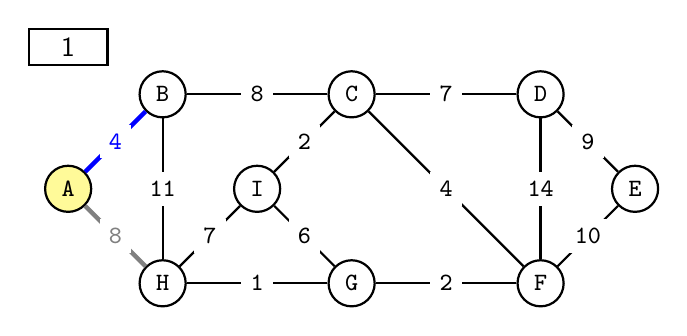
\begin{tikzpicture}[
        scale=1,
        transform shape,
        thick,
        font=\ttfamily\bfseries\small
    ]
    \tikzset{
        mynode/.style = {circle, draw=black, align=center,fill=white},
        mynodeb/.style = {circle, draw=black, align=center,fill=yellow!40},
        edgen/.style = {-},
        edger/.style = {-,ultra thick,red},
        edgeb/.style = {-,ultra thick,blue},
        edgeg/.style = {-,ultra thick,gray},
    }
    \node[rectangle,draw=black,font=\sffamily, minimum width=1cm] at (0.0,3.0) {1};
    \node[mynodeb] at (0.0,1.2) (a) {A};
    \node[mynode] at (1.2,2.4) (b) {B};
    \node[mynode] at (6.0,2.4) (d) {D};
    \node[mynode] at (3.6,2.4) (c) {C};
    \node[mynode] at (1.2,0.0) (h) {H};
    \node[mynode] at (3.6,0.0) (g) {G};
    \node[mynode] at (6.0,0.0) (f) {F};
    \node[mynode] at (2.4,1.2) (i) {I};
    \node[mynode] at (7.2,1.2) (e) {E};
    %
    \draw[edgeb] (a) edge node[fill=white] {4} (b);
    \draw[edgen] (b) edge node[fill=white] {8} (c);
    \draw[edgen] (c) edge node[fill=white] {7} (d);
    \draw[edgen] (d) edge node[fill=white] {9} (e);
    %
    \draw[edgeg] (a) edge node[fill=white] {8} (h);
    \draw[edgen] (h) edge node[fill=white] {1} (g);
    \draw[edgen] (g) edge node[fill=white] {2} (f);
    \draw[edgen] (f) edge node[fill=white] {10} (e);
    %
    \draw[edgen] (h) edge node[fill=white] {7} (i);
    \draw[edgen] (i) edge node[fill=white] {6} (g);
    \draw[edgen] (i) edge node[fill=white] {2} (c);
    %
    \draw[edgen] (b) edge node[fill=white] {11} (h);
    \draw[edgen] (d) edge node[fill=white] {14} (f);
    \draw[edgen] (c) edge node[fill=white] {4} (f);
    \end{tikzpicture}
\end{page}

\begin{page}
    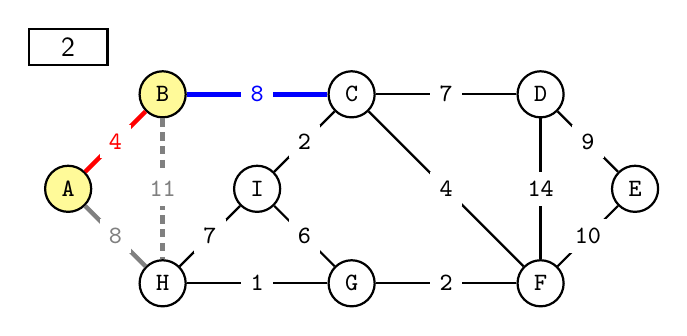
\begin{tikzpicture}[
        scale=1,
        transform shape,
        thick,
        font=\ttfamily\bfseries\small
    ]
    \tikzset{
        mynode/.style = {circle, draw=black, align=center,fill=white},
        mynodeb/.style = {circle, draw=black, align=center,fill=yellow!40},
        edgen/.style = {-},
        edger/.style = {-,ultra thick,red},
        edgeb/.style = {-,ultra thick,blue},
        edgeg/.style = {-,ultra thick,gray},
        edgegg/.style = {-,ultra thick,gray,densely dashed},
    }
    \node[rectangle,draw=black,font=\sffamily, minimum width=1cm] at (0.0,3.0) {2};
    \node[mynodeb] at (0.0,1.2) (a) {A};
    \node[mynodeb] at (1.2,2.4) (b) {B};
    \node[mynode] at (6.0,2.4) (d) {D};
    \node[mynode] at (3.6,2.4) (c) {C};
    \node[mynode] at (1.2,0.0) (h) {H};
    \node[mynode] at (3.6,0.0) (g) {G};
    \node[mynode] at (6.0,0.0) (f) {F};
    \node[mynode] at (2.4,1.2) (i) {I};
    \node[mynode] at (7.2,1.2) (e) {E};
    %
    \draw[edger] (a) edge node[fill=white] {4} (b);
    \draw[edgeb] (b) edge node[fill=white] {8} (c);
    \draw[edgen] (c) edge node[fill=white] {7} (d);
    \draw[edgen] (d) edge node[fill=white] {9} (e);
    %
    \draw[edgeg] (a) edge node[fill=white] {8} (h);
    \draw[edgen] (h) edge node[fill=white] {1} (g);
    \draw[edgen] (g) edge node[fill=white] {2} (f);
    \draw[edgen] (f) edge node[fill=white] {10} (e);
    %
    \draw[edgen] (h) edge node[fill=white] {7} (i);
    \draw[edgen] (i) edge node[fill=white] {6} (g);
    \draw[edgen] (i) edge node[fill=white] {2} (c);
    %
    \draw[edgegg] (b) edge node[fill=white] {11} (h);
    \draw[edgen] (d) edge node[fill=white] {14} (f);
    \draw[edgen] (c) edge node[fill=white] {4} (f);
    \end{tikzpicture}
\end{page}

\begin{page}
    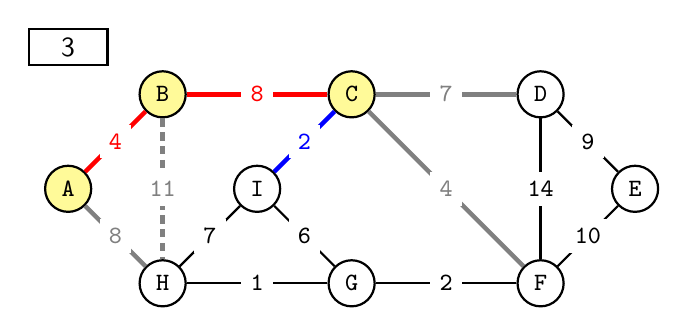
\begin{tikzpicture}[
        scale=1,
        transform shape,
        thick,
        font=\ttfamily\bfseries\small
    ]
    \tikzset{
        mynode/.style = {circle, draw=black, align=center,fill=white},
        mynodeb/.style = {circle, draw=black, align=center,fill=yellow!40},
        edgen/.style = {-},
        edger/.style = {-,ultra thick,red},
        edgeb/.style = {-,ultra thick,blue},
        edgeg/.style = {-,ultra thick,gray},
        edgegg/.style = {-,ultra thick,gray,densely dashed},
    }
    \node[rectangle,draw=black,font=\sffamily, minimum width=1cm] at (0.0,3.0) {3};
    \node[mynodeb] at (0.0,1.2) (a) {A};
    \node[mynodeb] at (1.2,2.4) (b) {B};
    \node[mynode] at (6.0,2.4) (d) {D};
    \node[mynodeb] at (3.6,2.4) (c) {C};
    \node[mynode] at (1.2,0.0) (h) {H};
    \node[mynode] at (3.6,0.0) (g) {G};
    \node[mynode] at (6.0,0.0) (f) {F};
    \node[mynode] at (2.4,1.2) (i) {I};
    \node[mynode] at (7.2,1.2) (e) {E};
    %
    \draw[edger] (a) edge node[fill=white] {4} (b);
    \draw[edger] (b) edge node[fill=white] {8} (c);
    \draw[edgeg] (c) edge node[fill=white] {7} (d);
    \draw[edgen] (d) edge node[fill=white] {9} (e);
    %
    \draw[edgeg] (a) edge node[fill=white] {8} (h);
    \draw[edgen] (h) edge node[fill=white] {1} (g);
    \draw[edgen] (g) edge node[fill=white] {2} (f);
    \draw[edgen] (f) edge node[fill=white] {10} (e);
    %
    \draw[edgen] (h) edge node[fill=white] {7} (i);
    \draw[edgen] (i) edge node[fill=white] {6} (g);
    \draw[edgeb] (i) edge node[fill=white] {2} (c);
    %
    \draw[edgegg] (b) edge node[fill=white] {11} (h);
    \draw[edgen] (d) edge node[fill=white] {14} (f);
    \draw[edgeg] (c) edge node[fill=white] {4} (f);
    \end{tikzpicture}
\end{page}

\begin{page}
    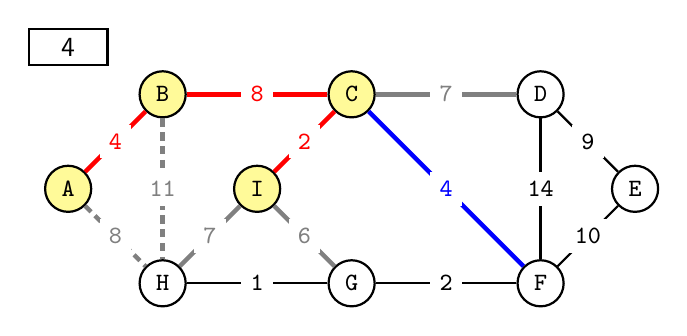
\begin{tikzpicture}[
        scale=1,
        transform shape,
        thick,
        font=\ttfamily\bfseries\small
    ]
    \tikzset{
        mynode/.style = {circle, draw=black, align=center,fill=white},
        mynodeb/.style = {circle, draw=black, align=center,fill=yellow!40},
        edgen/.style = {-},
        edger/.style = {-,ultra thick,red},
        edgeb/.style = {-,ultra thick,blue},
        edgeg/.style = {-,ultra thick,gray},
        edgegg/.style = {-,ultra thick,gray,densely dashed},
    }
    \node[rectangle,draw=black,font=\sffamily, minimum width=1cm] at (0.0,3.0) {4};
    \node[mynodeb] at (0.0,1.2) (a) {A};
    \node[mynodeb] at (1.2,2.4) (b) {B};
    \node[mynode] at (6.0,2.4) (d) {D};
    \node[mynodeb] at (3.6,2.4) (c) {C};
    \node[mynode] at (1.2,0.0) (h) {H};
    \node[mynode] at (3.6,0.0) (g) {G};
    \node[mynode] at (6.0,0.0) (f) {F};
    \node[mynodeb] at (2.4,1.2) (i) {I};
    \node[mynode] at (7.2,1.2) (e) {E};
    %
    \draw[edger] (a) edge node[fill=white] {4} (b);
    \draw[edger] (b) edge node[fill=white] {8} (c);
    \draw[edgeg] (c) edge node[fill=white] {7} (d);
    \draw[edgen] (d) edge node[fill=white] {9} (e);
    %
    \draw[edgegg] (a) edge node[fill=white] {8} (h);
    \draw[edgen] (h) edge node[fill=white] {1} (g);
    \draw[edgen] (g) edge node[fill=white] {2} (f);
    \draw[edgen] (f) edge node[fill=white] {10} (e);
    %
    \draw[edgeg] (h) edge node[fill=white] {7} (i);
    \draw[edgeg] (i) edge node[fill=white] {6} (g);
    \draw[edger] (i) edge node[fill=white] {2} (c);
    %
    \draw[edgegg] (b) edge node[fill=white] {11} (h);
    \draw[edgen] (d) edge node[fill=white] {14} (f);
    \draw[edgeb] (c) edge node[fill=white] {4} (f);
    \end{tikzpicture}
\end{page}

\begin{page}
    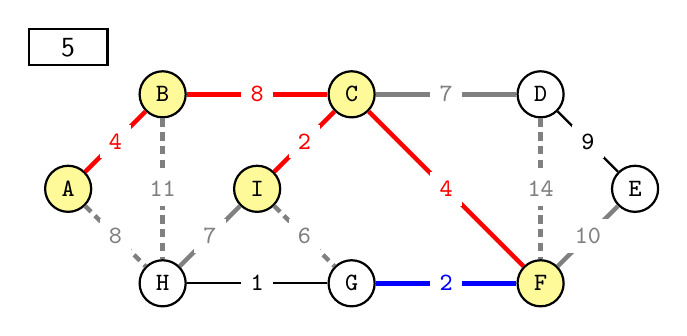
\begin{tikzpicture}[
        scale=1,
        transform shape,
        thick,
        font=\ttfamily\bfseries\small
    ]
    \tikzset{
        mynode/.style = {circle, draw=black, align=center,fill=white},
        mynodeb/.style = {circle, draw=black, align=center,fill=yellow!40},
        edgen/.style = {-},
        edger/.style = {-,ultra thick,red},
        edgeb/.style = {-,ultra thick,blue},
        edgeg/.style = {-,ultra thick,gray},
        edgegg/.style = {-,ultra thick,gray,densely dashed},
    }
    \node[rectangle,draw=black,font=\sffamily, minimum width=1cm] at (0.0,3.0) {5};
    \node[mynodeb] at (0.0,1.2) (a) {A};
    \node[mynodeb] at (1.2,2.4) (b) {B};
    \node[mynode] at (6.0,2.4) (d) {D};
    \node[mynodeb] at (3.6,2.4) (c) {C};
    \node[mynode] at (1.2,0.0) (h) {H};
    \node[mynode] at (3.6,0.0) (g) {G};
    \node[mynodeb] at (6.0,0.0) (f) {F};
    \node[mynodeb] at (2.4,1.2) (i) {I};
    \node[mynode] at (7.2,1.2) (e) {E};
    %
    \draw[edger] (a) edge node[fill=white] {4} (b);
    \draw[edger] (b) edge node[fill=white] {8} (c);
    \draw[edgeg] (c) edge node[fill=white] {7} (d);
    \draw[edgen] (d) edge node[fill=white] {9} (e);
    %
    \draw[edgegg] (a) edge node[fill=white] {8} (h);
    \draw[edgen] (h) edge node[fill=white] {1} (g);
    \draw[edgeb] (g) edge node[fill=white] {2} (f);
    \draw[edgeg] (f) edge node[fill=white] {10} (e);
    %
    \draw[edgeg] (h) edge node[fill=white] {7} (i);
    \draw[edgegg] (i) edge node[fill=white] {6} (g);
    \draw[edger] (i) edge node[fill=white] {2} (c);
    %
    \draw[edgegg] (b) edge node[fill=white] {11} (h);
    \draw[edgegg] (d) edge node[fill=white] {14} (f);
    \draw[edger] (c) edge node[fill=white] {4} (f);
    \end{tikzpicture}
\end{page}

\begin{page}
    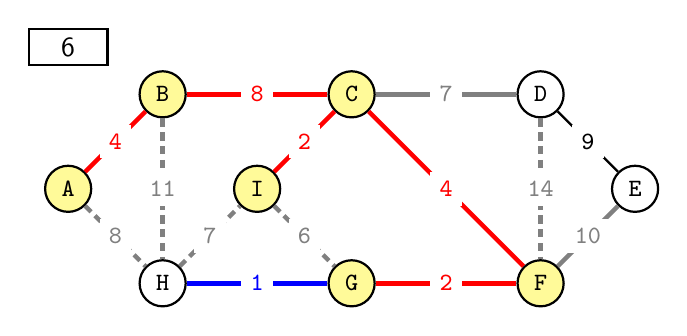
\begin{tikzpicture}[
        scale=1,
        transform shape,
        thick,
        font=\ttfamily\bfseries\small
    ]
    \tikzset{
        mynode/.style = {circle, draw=black, align=center,fill=white},
        mynodeb/.style = {circle, draw=black, align=center,fill=yellow!40},
        edgen/.style = {-},
        edger/.style = {-,ultra thick,red},
        edgeb/.style = {-,ultra thick,blue},
        edgeg/.style = {-,ultra thick,gray},
        edgegg/.style = {-,ultra thick,gray,densely dashed},
    }
    \node[rectangle,draw=black,font=\sffamily, minimum width=1cm] at (0.0,3.0) {6};
    \node[mynodeb] at (0.0,1.2) (a) {A};
    \node[mynodeb] at (1.2,2.4) (b) {B};
    \node[mynode] at (6.0,2.4) (d) {D};
    \node[mynodeb] at (3.6,2.4) (c) {C};
    \node[mynode] at (1.2,0.0) (h) {H};
    \node[mynodeb] at (3.6,0.0) (g) {G};
    \node[mynodeb] at (6.0,0.0) (f) {F};
    \node[mynodeb] at (2.4,1.2) (i) {I};
    \node[mynode] at (7.2,1.2) (e) {E};
    %
    \draw[edger] (a) edge node[fill=white] {4} (b);
    \draw[edger] (b) edge node[fill=white] {8} (c);
    \draw[edgeg] (c) edge node[fill=white] {7} (d);
    \draw[edgen] (d) edge node[fill=white] {9} (e);
    %
    \draw[edgegg] (a) edge node[fill=white] {8} (h);
    \draw[edgeb] (h) edge node[fill=white] {1} (g);
    \draw[edger] (g) edge node[fill=white] {2} (f);
    \draw[edgeg] (f) edge node[fill=white] {10} (e);
    %
    \draw[edgegg] (h) edge node[fill=white] {7} (i);
    \draw[edgegg] (i) edge node[fill=white] {6} (g);
    \draw[edger] (i) edge node[fill=white] {2} (c);
    %
    \draw[edgegg] (b) edge node[fill=white] {11} (h);
    \draw[edgegg] (d) edge node[fill=white] {14} (f);
    \draw[edger] (c) edge node[fill=white] {4} (f);
    \end{tikzpicture}
\end{page}

\begin{page}
    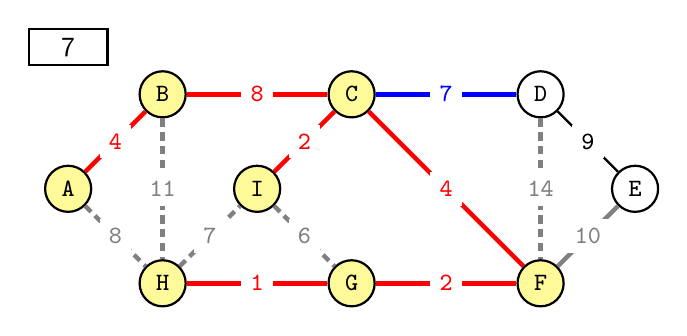
\begin{tikzpicture}[
        scale=1,
        transform shape,
        thick,
        font=\ttfamily\bfseries\small
    ]
    \tikzset{
        mynode/.style = {circle, draw=black, align=center,fill=white},
        mynodeb/.style = {circle, draw=black, align=center,fill=yellow!40},
        edgen/.style = {-},
        edger/.style = {-,ultra thick,red},
        edgeb/.style = {-,ultra thick,blue},
        edgeg/.style = {-,ultra thick,gray},
        edgegg/.style = {-,ultra thick,gray,densely dashed},
    }
    \node[rectangle,draw=black,font=\sffamily, minimum width=1cm] at (0.0,3.0) {7};
    \node[mynodeb] at (0.0,1.2) (a) {A};
    \node[mynodeb] at (1.2,2.4) (b) {B};
    \node[mynode] at (6.0,2.4) (d) {D};
    \node[mynodeb] at (3.6,2.4) (c) {C};
    \node[mynodeb] at (1.2,0.0) (h) {H};
    \node[mynodeb] at (3.6,0.0) (g) {G};
    \node[mynodeb] at (6.0,0.0) (f) {F};
    \node[mynodeb] at (2.4,1.2) (i) {I};
    \node[mynode] at (7.2,1.2) (e) {E};
    %
    \draw[edger] (a) edge node[fill=white] {4} (b);
    \draw[edger] (b) edge node[fill=white] {8} (c);
    \draw[edgeb] (c) edge node[fill=white] {7} (d);
    \draw[edgen] (d) edge node[fill=white] {9} (e);
    %
    \draw[edgegg] (a) edge node[fill=white] {8} (h);
    \draw[edger] (h) edge node[fill=white] {1} (g);
    \draw[edger] (g) edge node[fill=white] {2} (f);
    \draw[edgeg] (f) edge node[fill=white] {10} (e);
    %
    \draw[edgegg] (h) edge node[fill=white] {7} (i);
    \draw[edgegg] (i) edge node[fill=white] {6} (g);
    \draw[edger] (i) edge node[fill=white] {2} (c);
    %
    \draw[edgegg] (b) edge node[fill=white] {11} (h);
    \draw[edgegg] (d) edge node[fill=white] {14} (f);
    \draw[edger] (c) edge node[fill=white] {4} (f);
    \end{tikzpicture}
\end{page}

\begin{page}
    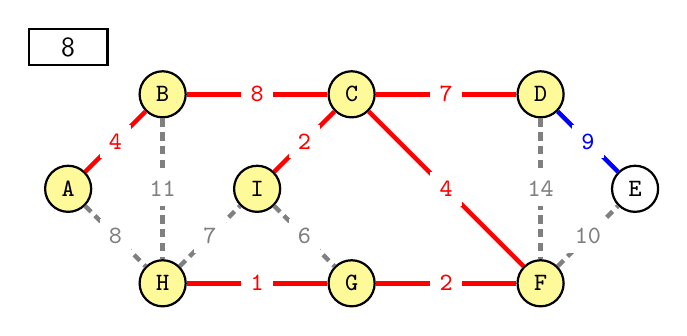
\begin{tikzpicture}[
        scale=1,
        transform shape,
        thick,
        font=\ttfamily\bfseries\small
    ]
    \tikzset{
        mynode/.style = {circle, draw=black, align=center,fill=white},
        mynodeb/.style = {circle, draw=black, align=center,fill=yellow!40},
        edgen/.style = {-},
        edger/.style = {-,ultra thick,red},
        edgeb/.style = {-,ultra thick,blue},
        edgeg/.style = {-,ultra thick,gray},
        edgegg/.style = {-,ultra thick,gray,densely dashed},
    }
    \node[rectangle,draw=black,font=\sffamily, minimum width=1cm] at (0.0,3.0) {8};
    \node[mynodeb] at (0.0,1.2) (a) {A};
    \node[mynodeb] at (1.2,2.4) (b) {B};
    \node[mynodeb] at (6.0,2.4) (d) {D};
    \node[mynodeb] at (3.6,2.4) (c) {C};
    \node[mynodeb] at (1.2,0.0) (h) {H};
    \node[mynodeb] at (3.6,0.0) (g) {G};
    \node[mynodeb] at (6.0,0.0) (f) {F};
    \node[mynodeb] at (2.4,1.2) (i) {I};
    \node[mynode] at (7.2,1.2) (e) {E};
    %
    \draw[edger] (a) edge node[fill=white] {4} (b);
    \draw[edger] (b) edge node[fill=white] {8} (c);
    \draw[edger] (c) edge node[fill=white] {7} (d);
    \draw[edgeb] (d) edge node[fill=white] {9} (e);
    %
    \draw[edgegg] (a) edge node[fill=white] {8} (h);
    \draw[edger] (h) edge node[fill=white] {1} (g);
    \draw[edger] (g) edge node[fill=white] {2} (f);
    \draw[edgegg] (f) edge node[fill=white] {10} (e);
    %
    \draw[edgegg] (h) edge node[fill=white] {7} (i);
    \draw[edgegg] (i) edge node[fill=white] {6} (g);
    \draw[edger] (i) edge node[fill=white] {2} (c);
    %
    \draw[edgegg] (b) edge node[fill=white] {11} (h);
    \draw[edgegg] (d) edge node[fill=white] {14} (f);
    \draw[edger] (c) edge node[fill=white] {4} (f);
    \end{tikzpicture}
\end{page}

\begin{page}
    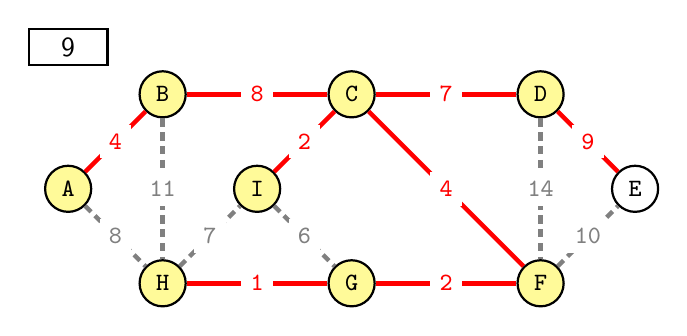
\begin{tikzpicture}[
        scale=1,
        transform shape,
        thick,
        font=\ttfamily\bfseries\small
    ]
    \tikzset{
        mynode/.style = {circle, draw=black, align=center,fill=white},
        mynodeb/.style = {circle, draw=black, align=center,fill=yellow!40},
        edgen/.style = {-},
        edger/.style = {-,ultra thick,red},
        edgeb/.style = {-,ultra thick,blue},
        edgeg/.style = {-,ultra thick,gray},
        edgegg/.style = {-,ultra thick,gray,densely dashed},
    }
    \node[rectangle,draw=black,font=\sffamily, minimum width=1cm] at (0.0,3.0) {9};
    \node[mynodeb] at (0.0,1.2) (a) {A};
    \node[mynodeb] at (1.2,2.4) (b) {B};
    \node[mynodeb] at (6.0,2.4) (d) {D};
    \node[mynodeb] at (3.6,2.4) (c) {C};
    \node[mynodeb] at (1.2,0.0) (h) {H};
    \node[mynodeb] at (3.6,0.0) (g) {G};
    \node[mynodeb] at (6.0,0.0) (f) {F};
    \node[mynodeb] at (2.4,1.2) (i) {I};
    \node[mynode] at (7.2,1.2) (e) {E};
    %
    \draw[edger] (a) edge node[fill=white] {4} (b);
    \draw[edger] (b) edge node[fill=white] {8} (c);
    \draw[edger] (c) edge node[fill=white] {7} (d);
    \draw[edger] (d) edge node[fill=white] {9} (e);
    %
    \draw[edgegg] (a) edge node[fill=white] {8} (h);
    \draw[edger] (h) edge node[fill=white] {1} (g);
    \draw[edger] (g) edge node[fill=white] {2} (f);
    \draw[edgegg] (f) edge node[fill=white] {10} (e);
    %
    \draw[edgegg] (h) edge node[fill=white] {7} (i);
    \draw[edgegg] (i) edge node[fill=white] {6} (g);
    \draw[edger] (i) edge node[fill=white] {2} (c);
    %
    \draw[edgegg] (b) edge node[fill=white] {11} (h);
    \draw[edgegg] (d) edge node[fill=white] {14} (f);
    \draw[edger] (c) edge node[fill=white] {4} (f);
    \end{tikzpicture}
\end{page}

\end{document}